\documentclass[12pt,a4paper]{article}
\usepackage[utf8]{inputenc}
\usepackage[german]{babel}
\usepackage[T1]{fontenc}
\usepackage{amsmath}
\usepackage{amsfonts}
\usepackage{amssymb}
\usepackage{graphicx}
\usepackage{siunitx}
\usepackage{float}
\usepackage[left=2cm,right=2cm,top=2cm,bottom=2cm]{geometry}
\author{Gerald}

\begin{document}
\sisetup{separate-uncertainty = true}
	\setlength{\parindent}{0pt} 
	\begin{center}
		{\LARGE Versuchsprotokoll}\\
		\begin{large}
			zum Fortgeschrittenenpraktikum im Bachelorstudiengang Physik\\[0.4cm]
			an der RWTH Aachen\\
			II. Physikalisches Institut A\\[5.5cm]
			\Large\textbf{\textsl{Gasdetektoren und Statistik (T07)}}\\[5.5cm]
			\normalsize\textit{vorgelegt\\von}\\[0.4cm]
			\large{Moritz Berger (355244)\\Gerald Kolter (355005)}\\[2cm]
			\large \textbf{Wintersemester 2017/18}
		\end{large}
	\end{center}
	\newpage
	
	\tableofcontents
	\newpage
	
	
\section{Versuchsziel}
Das Ziel dieses Versuches ist in zwei Teile aufgeteilt.\\
Als erstes sollen die Eigenschaften eines Proportionalzählers und eines Geiger-Müller-Zählrohres untersucht werden. Dazu wird zum einen die Charakteristik, also die Abhängigkeit der Zählrate von der angelegten Spannung, untersucht, um den optimalen Bereich für die Betriebsspannung zu erhalten. Es wird außerdem die Abhängigkeit der Stärke eines Pulses des Proportionalzählers von der Spannung betrachtet und die Tot- und  Erhohlzeit des Geiger-Müller-Zählers bestimmt.\\
Im zweiten Versuchsteil sollen Messungen durchgeführt werden, die verschiedene vorhergesagte Verteilungen bestätigen. Dabei soll eine Gaussverteilung für eine hohe Anzahl an Messungen, eine Poissonverteilung für kleine Messergebnisse und eine Exponetialverteilung für den Abstand zwischen zwei gemessenen Zerfällen untersucht werden. 
\section{Aufbau}
\subsection{Geiger-Müller-Zählrohr}
\subsection{Proportionalzähler}

\section{Durchführung}
\subsection{Geiger-Müller-Zählrohr}
\subsubsection{Charakteristik}
Die Charakteristik wird mithilfe des $_{38}^{90}Sr$-Präparates gemessen. Dabei wird bei eingebrachtem Präparat die Spannung, ausgehend von der Minimaleinstellung von \SI{250}{V}, in \SI{10}{V} erhöht und jeweils über \SI{10}{s} die Anzahl der gemessenen Ereignisse erfasst.\\
Um die Einsatzspannung $U_E$ und die Geiger-Schwelle $U_G$ genauer bestimmen zu können, wurde im entsprechenden Bereich, in dem sich diese Werte befinden, in \SI{2}{V} Schritten statt in \SI{10}{V} Schritten gemessen.
\subsubsection{Totzeit}
Die Totzeit wird über zwei verschiedene Methoden bestimmt.\\
Als erstes wird ein Stever-Diagramm erstellt, an dem man die Tod- und Erhohlungszeit ablesen kann.\\
Als zweites wird sie über eine Totzeitstufe bestimmt.
\subsection{Proportionalzähler}
\subsection{Statistikmessung}
Die Statistikmessungen wurden alle mit dem Geiger-Müller-Zählrohr aufgenommen.
\subsubsection{Poissonverteilung}
Die Zerfälle sind poissonverteilt. Um eine Poissonverteilung auch in den Messdaten beobachten zu können, muss die Messzeit klein gehalten werden (T = 0.3s), da die Verteilung ansonsten in eine Gaußverteilung übergeht. Die Poissonverteilung ist nur für diskrete Werte definiert und hat die Form:
\begin{equation}
P(n) = \dfrac{\mu ^n}{n!} \cdot e^{-\mu}
\end{equation}
\subsubsection{Gaußverteilung}
Da die Zerfälle poissonverteilt sind, muss für die Messung einer Gaußverteilung die Messzeit um Faktor 10 erhöht werden (T = 3s). Die Gaußverteilung hat die Form:
\begin{equation}
P(x) = \dfrac{1}{\sqrt{2 \pi} \sigma} \cdot e^{\frac{(x - \mu)^2}{2 \cdot \sigma ^2}}
\end{equation}
\subsubsection{Exponentialverteilung}
Die Abstände zwischen zwei Zerfällen sind exponentialverteilt. Zur Messung werden mit dem Oszilloskop Bilder gemacht, auf denen mehrere Zerfälle zu sehen sind. Die Exponentialverteilung hat die Form:
\begin{equation}
P(\Delta t) = A \cdot e^{- A \Delta t}
\end{equation}

\section{Ergebnisse}
\subsection{Geiger-Müller-Zählrohr}
\subsubsection{Charakteristik}
\subsubsection{Totzeit}
\subsection{Proportionalzähler}
\subsection{Statistikmessung}

\subsubsection{Poissonverteilung}
\begin{figure}
\centering
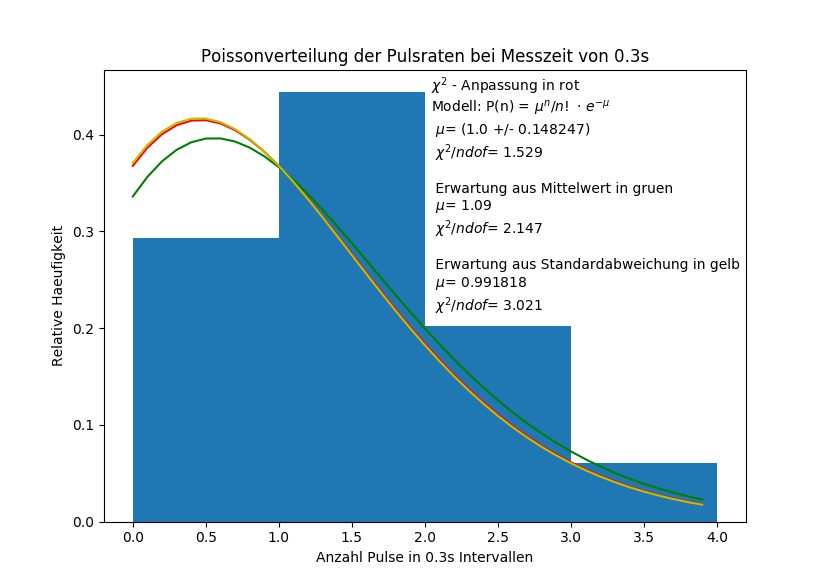
\includegraphics[scale=0.8]{Bilder/poisson.PNG}
\caption{Darstellung der gemessenen Poissonverteilung mit den Erwartungen und der Anpassung.}
\label{fig:Poisson}
\end{figure}

\begin{table}
\centering
\begin{tabular}{|c|c|c|c|}
\hline 
Art & Poisson Parameter & $\chi ^2$ /ndof & P($\chi ^2$) \\ 
\hline 
Mittelwertbestimmung & 1,0900 & 45,850 & 0\% \\ 
\hline 
Bestimmung der Standardabweichung & 0,9918 & 45,827 & 0\% \\ 
\hline 
$\chi ^2$ Anpassung & 0,9332 $\pm$ 0,3689 & 11,125 & 0\% \\ 
\hline 
\end{tabular} 
\caption{Poisson Parameter und $\chi ^2$ aus den verschiedenen Bestimmungsmethoden der Poissonverteilung. In der letzten Spalte ist eine geschätzte Wahrscheinlichkeit für den Wert des $\chi ^2$ angegeben.}
\label{tab:Poisson}
\end{table}

Für die Poissonverteilung wird die Anzahl der Pulse im Geiger-Müller-Zählrohr für ein festgelegtes Messintervall wiederholt gemessen. Die auftretenden Anzahlen werden dann in Intervalle mit Breite 1 zusammengefasst und aufgetragen. Das Ergebnis zeigt das Histogramm in Abbildung \ref{fig:Poisson} zusammen mit der $\chi ^2$ Anpassung (in rot) und den Erwartungen die sich aus der Bestimmung des Mittelwertes (grün) und der Standardabweichung (gelb) ergeben.\\
Für die Anpassung wurde auf jeden Wert ein Fehler gemäß der Poissonverteilung angenommen:
\begin{equation*}
\sigma _{n} = \sqrt{n}
\end{equation*}
Für die Anpassung einer Gaußverteilung wurden die Werte normiert, daher pflanzt sich der Fehler fort zu:
\begin{equation*}
n_{i, norm} = \dfrac{n_i}{\sum _j n_j} =: \dfrac{n_i}{N}
\end{equation*}
\begin{equation*}
\sigma _{i, norm} = \sqrt{ \sum _j \left( \sigma_j \cdot \left( \delta_{ij} \cdot \left( \frac{1}{N} - \frac{n_i}{N} \right) + (1 - \delta_{ij}) \cdot \frac{n_i}{N^2} \right) \right)^2 }
\end{equation*}
AB HIER POISSON ÜBERARBEITEN!! \\
Tabelle \ref{tab:Poisson} zeigt die Ergebnisse aus den verschiedenen Methoden zur Bestimmung des Poisson Parameters und des $\chi ^2$. Leicht lässt sich ersehen, dass die Werte für den Poisson Parameter nah beieinander liegen, das $\chi ^2$ aus der Anpassung jedoch deutlich kleiner ist als die aus der Berechnung nach Bestimmung des Parameters. Insgesamt ist das $\chi ^2$ jedoch deutlich zu groß. 


\subsubsection{Gaußverteilung}
\begin{figure}
\centering
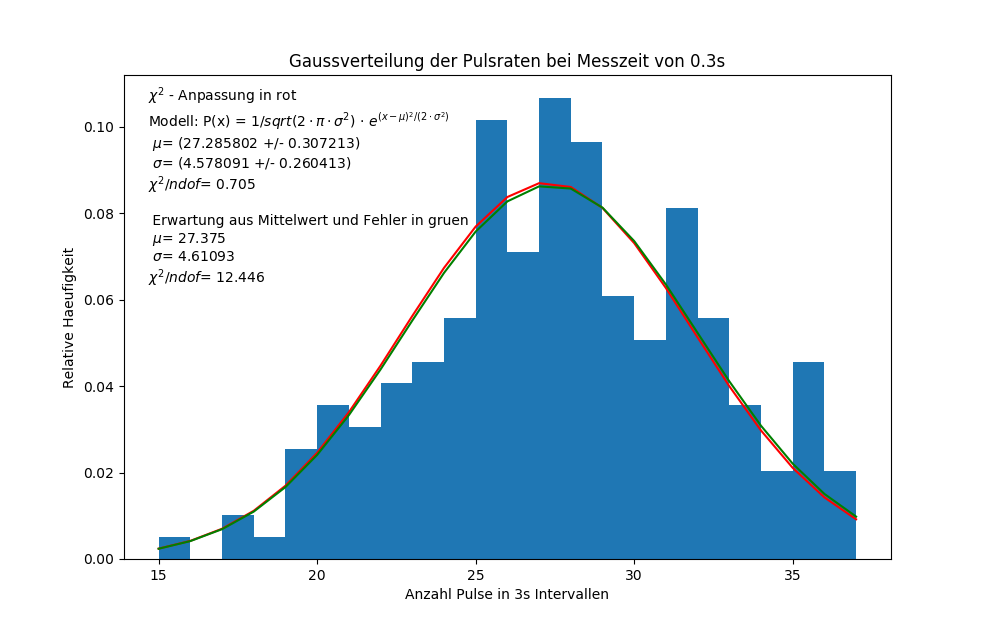
\includegraphics[scale=0.8]{Bilder/gauss.PNG}
\caption{Darstellung der gemessenen Gaußverteilung mit der Erwartung und der Anpassung.}
\label{fig:gauss}
\end{figure}

\begin{table}
\centering
\begin{tabular}{|c|c|c|c|c|}
\hline 
Art & Mittelwert & Standardabweichung & $\chi ^2$ /ndof & P($\chi ^2$) \\ 
\hline 
Bestimmung von $\sigma$ und $\mu$ & 27,375 & 4,611 & 0,688 & 30\% \\ 
\hline 
$\chi ^2$ Anpassung & 27,286 $\pm$ 0,307 & 4,578 $\pm$ 0,260 & 0,705 & 30\% \\ 
\hline 
\end{tabular} 
\caption{Mittelwert, Standardabweichung und $\chi ^2$ aus den verschiedenen Bestimmungsmethoden der Gaußverteilung. In der letzten Spalte ist eine geschätzte Wahrscheinlichkeit für den Wert des $\chi ^2$ angegeben.}
\label{tab:Gauss}
\end{table}

Das Verfahren bei der Gaußverteilung ist identisch zu dem Verfahren bei der Poissonverteilung. Es wurde auch die gleiche Fehlerabschätzung verwendet. Abbildung \ref{fig:gauss} zeigt das Ergebnis. Hier ist in rot die $\chi ^2$ Anpassung und die Erwartung aus Mittelwert und Standardabweichung in grün. In diesem Fall gibt es nur eine Erwartung, weil für die Bestimmung der Gaußverteilung Mittelwert und Standardabweichung notwendig sind.\\
Tabelle \ref{tab:Gauss} zeigt die Werte für Mittelwert, Standardabweichung und $\chi ^2$, die sich aus dem Fit und aus der Erwartung durch Bestimmung von Standardabweichung und Mittelwert ergibt. Die Werte für Mittelwert und Standardabweichung stimmen sehr gut überein und die $\chi ^2$ liegen ebenfalls sehr nah beieinander. Die Wahrscheinlichkeit für ein $\chi ^2$ pro Freiheitsgrad von 0,7 liegt ungefähr bei 30\%, daher kann von einer guten Messung gesprochen werden.


\subsubsection{Exponentialverteilung}
\begin{figure}
\centering
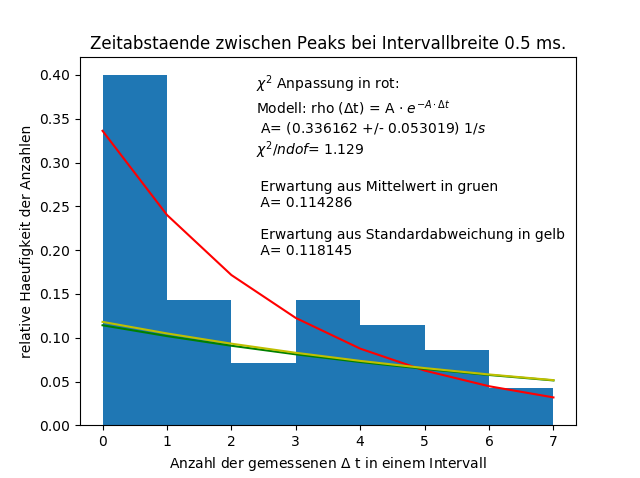
\includegraphics[scale=0.8]{Bilder/Peakabstaende.PNG}
\caption{Darstellung der gemessenen Peakabstände mit den Erwartungen und der Anpassung.}
\label{fig:exponential}
\end{figure}

\begin{table}
\centering
\begin{tabular}{|c|c|c|c|}
\hline 
Art & Exponentialparameter & $\chi ^2$ /ndof & P($\chi ^2$) \\ 
\hline 
Bestimmung von $\mu$ & 0,1143 & 11,307 & 0\% \\ 
\hline 
Bestimmung von $\sigma$ & 0,1181 & 11,302 & 0\% \\ 
\hline 
$\chi ^2$ Anpassung & 0,3362 $\pm$ 0,053 & 1,129 & 22\% \\ 
\hline 
\end{tabular} 
\caption{Exponential Parameter und $\chi ^2$ aus den verschiedenen Bestimmungsmethoden der Exponentialverteilung. In der letzten Spalte ist eine geschätzte Wahrscheinlichkeit für den Wert des $\chi ^2$ angegeben.}
\label{tab:Exponential}
\end{table}

Für die Auswertung der Exponentialverteilung werden die gemessenen Zeitabstände zunächst in sinnvolle Intervalle zusammengefasst. Die Anzahl der gemessenen $\Delta t$, die in diesem Intervall liegen werden auf die x-Achse aufgetragen. Die Anzahl der Intervalle mit der gleichen Anzahl der gemessenen $\Delta t$ wird auf die y-Achse aufgetragen. Dabei wird wieder normiert, daher kann wieder die gleiche Fehlerabschätzung wie bei der Poissonverteilung verwendet werden. Abbildung \ref{fig:exponential} zeigt das Ergebnis. Hier gibt es wieder zwei Erwartungen aus Bestimmung des Mittelwertes (grün) und Bestimmung der Standardabweichung (gelb). Die $\chi ^2$ Anpassung ist wieder in rot eingezeichnet.\\
Tabelle \ref{tab:Exponential} zeigt die Ergebnisse für den Exponentialparameter und das $\chi ^2$ pro Freiheitsgrad für die verschiedenen Bestimmungsmethoden. Auffällig ist, dass die Exponentialparameter aus den Bestimmungen von Mittelwert und Standardabweichung nah beieinander liegen, der Wert aus der $\chi ^2$ Anpassung jedoch deutlich von diesen abweicht. Das $\chi ^2$ ist bei der Anpassung deutlich besser, als bei den Bestimmungen von Mittelwert und Standardabweichung, sodass davon ausgegangen werden kann, dass der Wert aus der Anpassung näher am echten Wert liegt.

\section{Zusammenfassung}




	
\end{document}